% !TEX root = ../main.tex
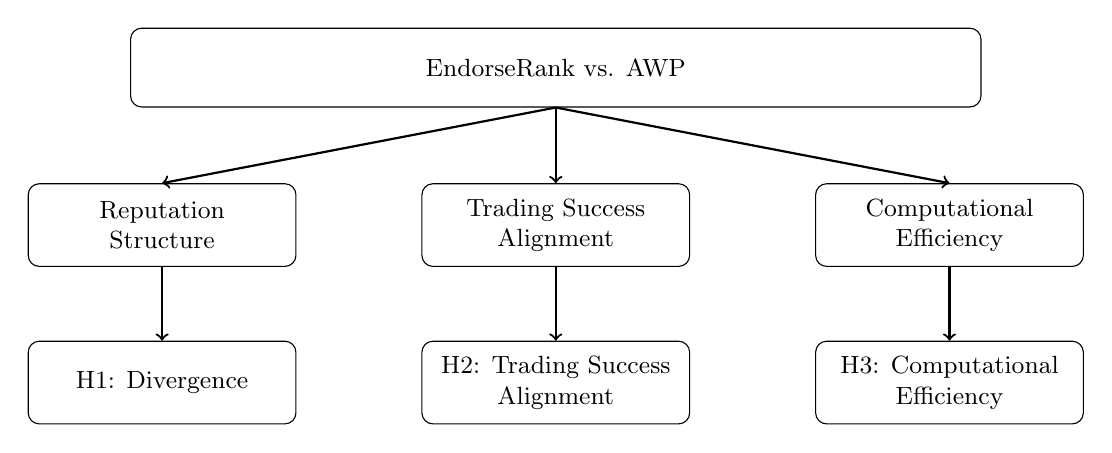
\begin{tikzpicture}[
  font=\small,
  box/.style={draw, rounded corners, align=center, minimum width=10.8cm, minimum height=1.0cm},
  smallbox/.style={draw, rounded corners, align=center, minimum width=3.4cm, minimum height=1.05cm},
  arrow/.style={->, thick}
]
\node[box] (center) at (0,2.6) {EndorseRank vs. AWP};

\node[smallbox] (rep) at (-5,0.6) {Reputation\\Structure};
\node[smallbox] (risk) at (0,0.6) {Trading Success\\Alignment};
\node[smallbox] (eff) at (5,0.6) {Computational\\Efficiency};

\node[smallbox] (h1) at (-5,-1.4) {H1: Divergence};
\node[smallbox] (h2) at (0,-1.4) {H2: Trading Success\\Alignment};
\node[smallbox] (h3) at (5,-1.4) {H3: Computational\\Efficiency};

\draw[arrow] (center.south) -- (rep.north);
\draw[arrow] (center.south) -- (risk.north);
\draw[arrow] (center.south) -- (eff.north);

\draw[arrow] (rep.south) -- (h1.north);
\draw[arrow] (risk.south) -- (h2.north);
\draw[arrow] (eff.south) -- (h3.north);
\end{tikzpicture}
